%!TEX root = thesis.tex

\chapter{Follow-Up User Study}
\label{chap:follow-up-user-study}

A follow-up user study was conducted to evaluate the set of refined visualisations. In addition to evaluating this iteration of the visualisation prototype, the limitations identified in the first user study were also to be addressed. This included providing a valid baseline for the study (the \emph{no visualisation} condition) and reducing the visualisations to more meaningful representations.

% The previous visualisation prototype and user study also lacked a clear baseline.  with an analysis and comparison to a live coded performance without -previous study did not have a baseline - this was to be remedied

It was hypothesised that the visualisation prototype would result in higher understanding at the end of the performance and that enjoyment would remain steady throughout both performances.

\section{Method}

Two independent audiences ($N=14+11=25$) were recruited through on campus advertisement (see Appendix~\ref{appendix:follow-up-user-study-advertisement}). Each group was exposed to two live coding musical performances. One of the performances displayed only the source code of the performance while the other displayed the source code with the refined visualisation prototype as an underlay (see Chapter~\ref{chap:visualisation-refinement}).

The first group was subjected to the \emph{visualisation} condition, followed by the \emph{no visualisation} condition. The conditions were swapped for the second group, with the audience exposed to the \emph{no visualisation} condition first followed by the \emph{visualisation} condition.

\section{Participants}

Of the 25 total participants over the two performances $12\%$ were female. $64\%$ of the audience had not been to a live coding performance before and $80\%$ had not attended the previous live coding user study. The background of the audience included $56\%$ that listened to music regularly, $28\%$ that played an instrument and $72\%$ who programmed for their hobby, job or study.

\section{Results}

The audience-reported enjoyment and understanding responses from the survey were evaluated for the two conditions as described below.

\subsection{Enjoyment}

$60\%$ of the audience stated that projection of the code helped their enjoyment of the performance directly while $16\%$ of the audience stated that the visualisations helped their enjoyment directly.

Levels of enjoyment throughout the performance were surveyed for the \emph{beginning}, \emph{middle} and the \emph{end} phases of the performance. A comparison of the enjoyment between the no visualisation condition and the visualisation condition is available in Figure~\ref{fig:no-visualisations-enjoyment} and Figure~\ref{fig:visualisations-enjoyment}.

Final levels of enjoyment between the two conditions differed only slightly. With no visualisation, $20\%$ stated that they had low enjoyment, $40\%$ stated that they had medium enjoyment and $40\%$ stated that they had high enjoyment. With visualisations, $20\%$ stated low enjoyment, $36\%$ stated medium enjoyment and $44\%$ stated high enjoyment.

\afterpage{
\begin{figure}
  \centering
  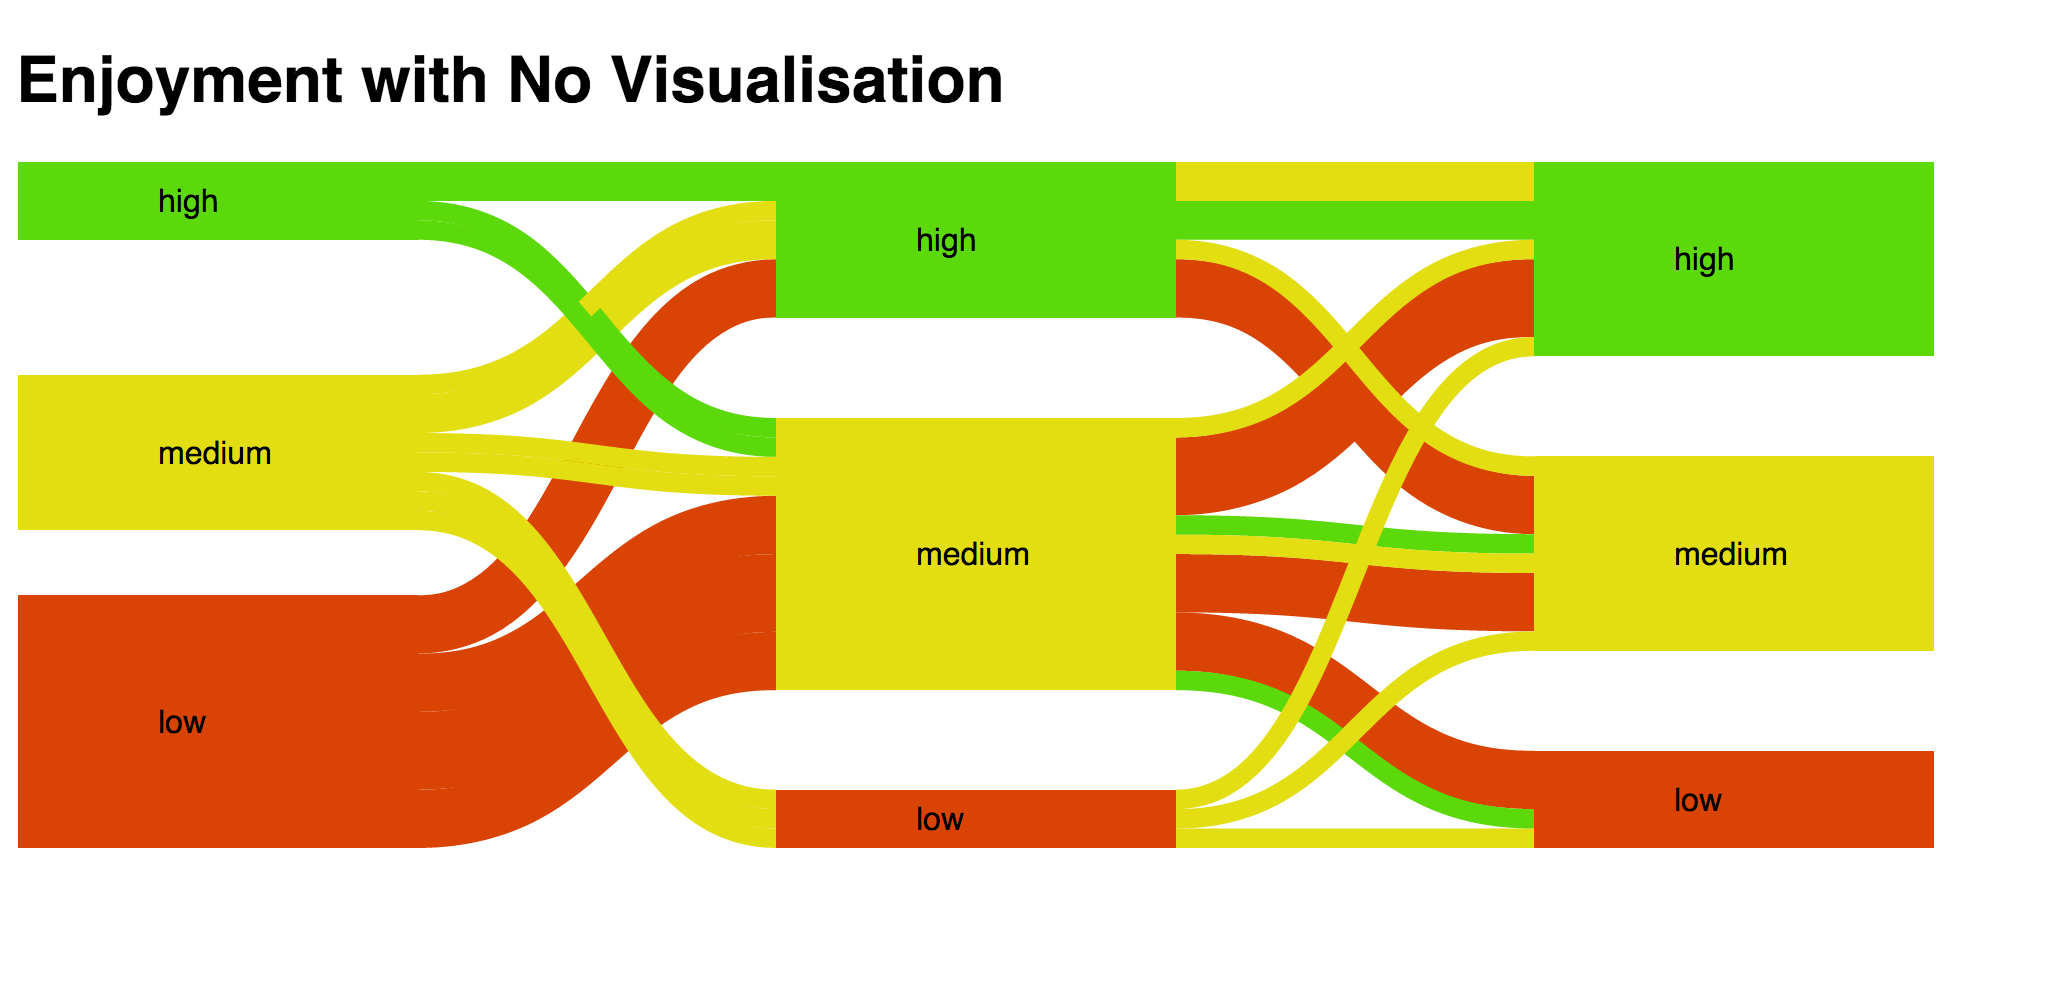
\includegraphics[width=\columnwidth]{../study-3/results/enjoyment-with-no-visualisation-study-3}
  \caption{Audience reported enjoyment during the beginning, middle and end of the performance with \textbf{no} visualisations. Line width at each stage indicates proportion of the audience reporting high, medium or low enjoyment, and line colour is determined by the enjoyment level at the \emph{beginning} of the performance.}
  \label{fig:no-visualisations-enjoyment}
\end{figure}

\begin{figure}
  \centering
  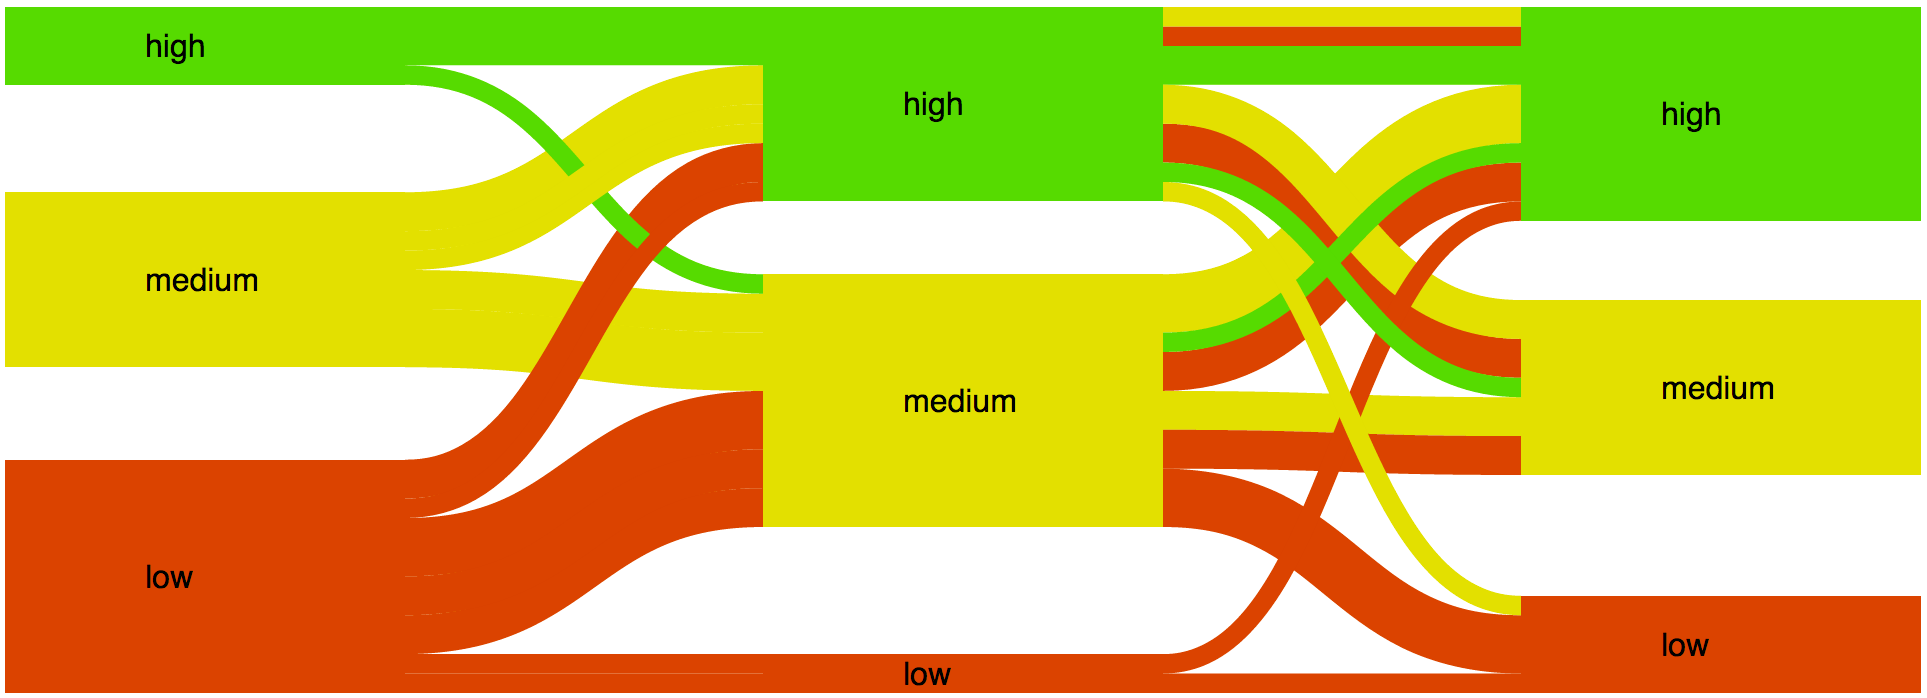
\includegraphics[width=\columnwidth]{../study-3/results/enjoyment-with-visualisation-study-3}
  \caption{Audience-reported enjoyment level during the beginning, middle and end of the performance with visualisations.}
  \label{fig:visualisations-enjoyment}
\end{figure}
\clearpage}

\subsection{Understanding}

$76\%$ of the audience stated that projection of the code helped their understanding of the performance directly while $32\%$ of the audience stated that the visualisations helped their understanding directly.

Levels of understanding throughout the performance were surveyed for the \emph{beginning}, \emph{middle} and the \emph{end} phases of the performance. A comparison of the understanding between the no visualisation condition and the visualisation condition is available in Figure~\ref{fig:no-visualisations-understanding} and Figure~\ref{fig:visualisations-understanding}.

Levels of understanding also differed slightly between the two conditions. With no visualisation, $32\%$ stated that they had low understanding, $48\%$ stated that they had medium understanding and $20\%$ stated that they had high understanding. With visualisations, $28\%$ stated low understanding, $44\%$ stated medium understanding and $28\%$ stated high understanding.

\afterpage{
\begin{figure}
  \centering
  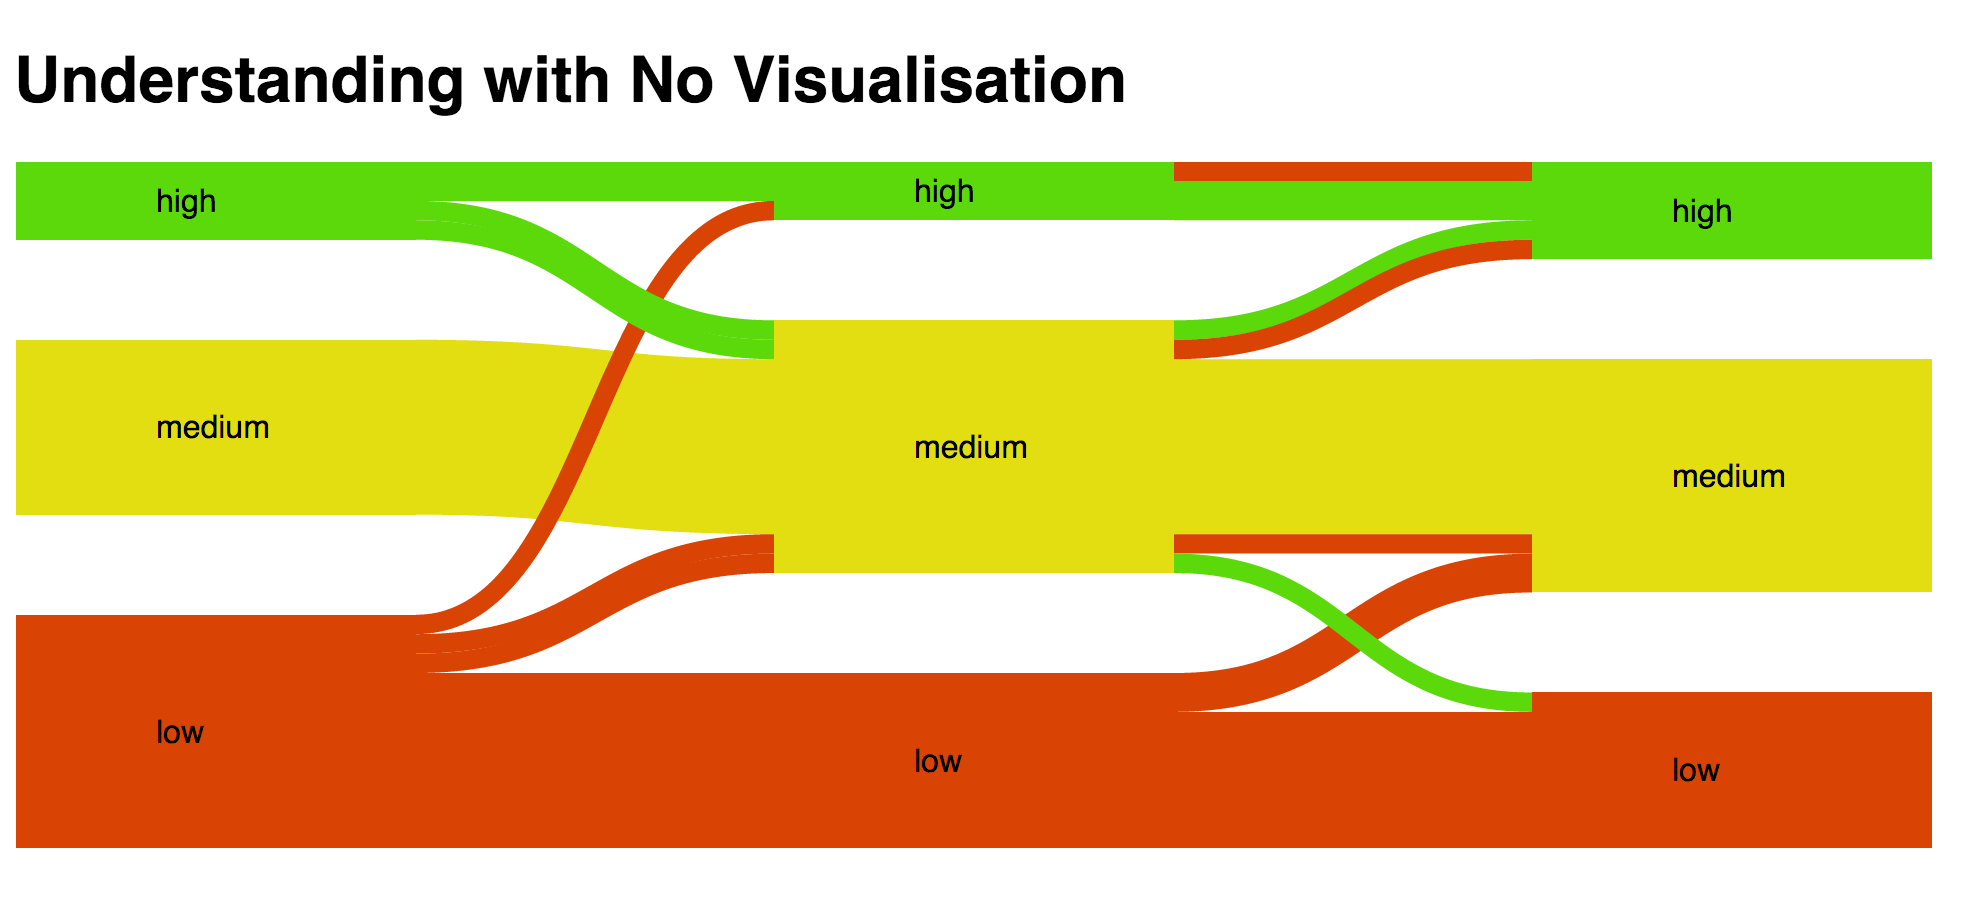
\includegraphics[width=\columnwidth]{../study-3/results/understanding-with-no-visualisation-study-3}
  \caption{Audience reported understanding during the beginning, middle and end of the performance with \textbf{no} visualisations.}
  \label{fig:no-visualisations-understanding}
\end{figure}

\begin{figure}
  \centering
  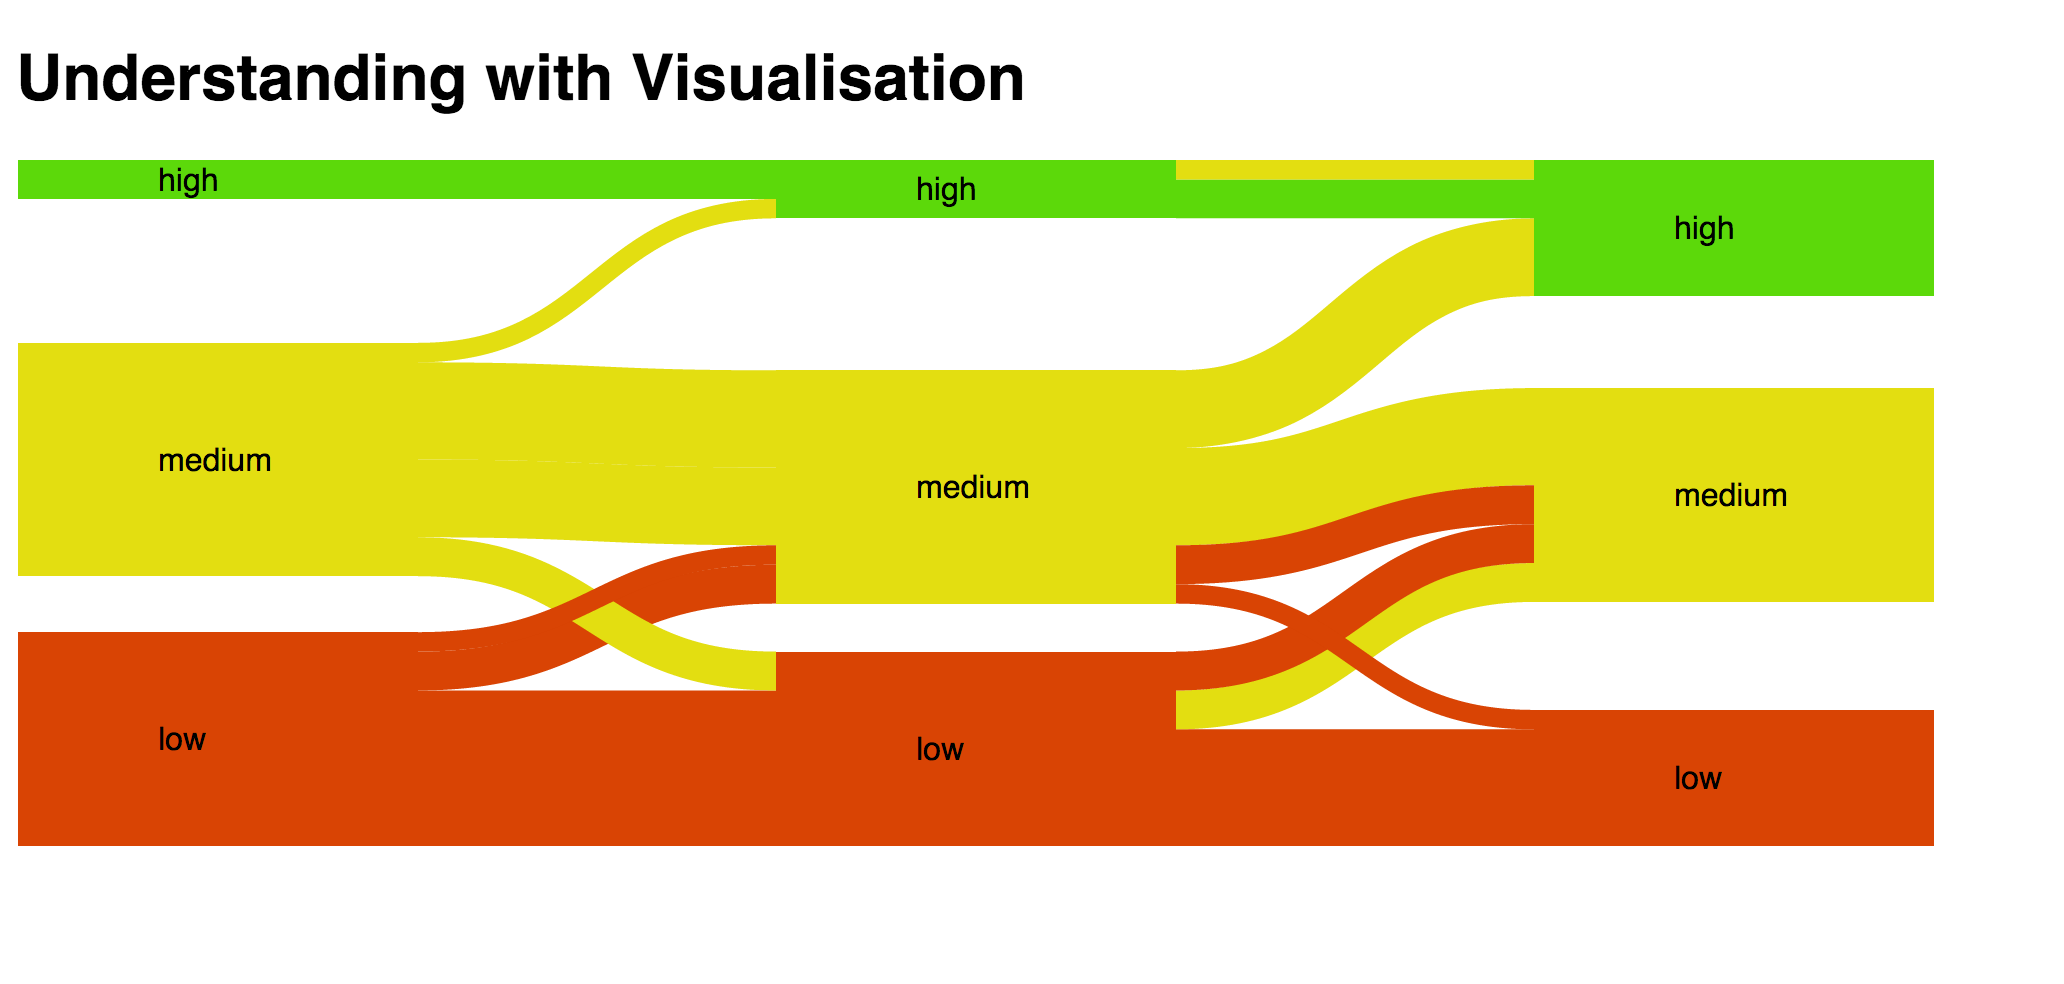
\includegraphics[width=\columnwidth]{../study-3/results/understanding-with-visualisation-study-3}
  \caption{Audience reported understanding during the beginning, middle and end of the performance with visualisations.}
  \label{fig:visualisations-understanding}
\end{figure}

\clearpage}

After each performance, two additional questions were asked. The additional questions were ``what do you think the performer was doing in the very early stages of the performance?'' and ``what do you think the performer was doing in the very last stages of the performance?''. Results from these questions were evaluated against a criteria for understanding level. {\color{red} discuss criteria here}


\subsection{Liveness}

After exposing the audience to both conditions, the audience was asked if the projected visualsations helped to communicate the feeling that the performances were live. Results of this question indicate that...

\more

\section{Discussion}

\afterpage{
\begin{figure}
  \centering
  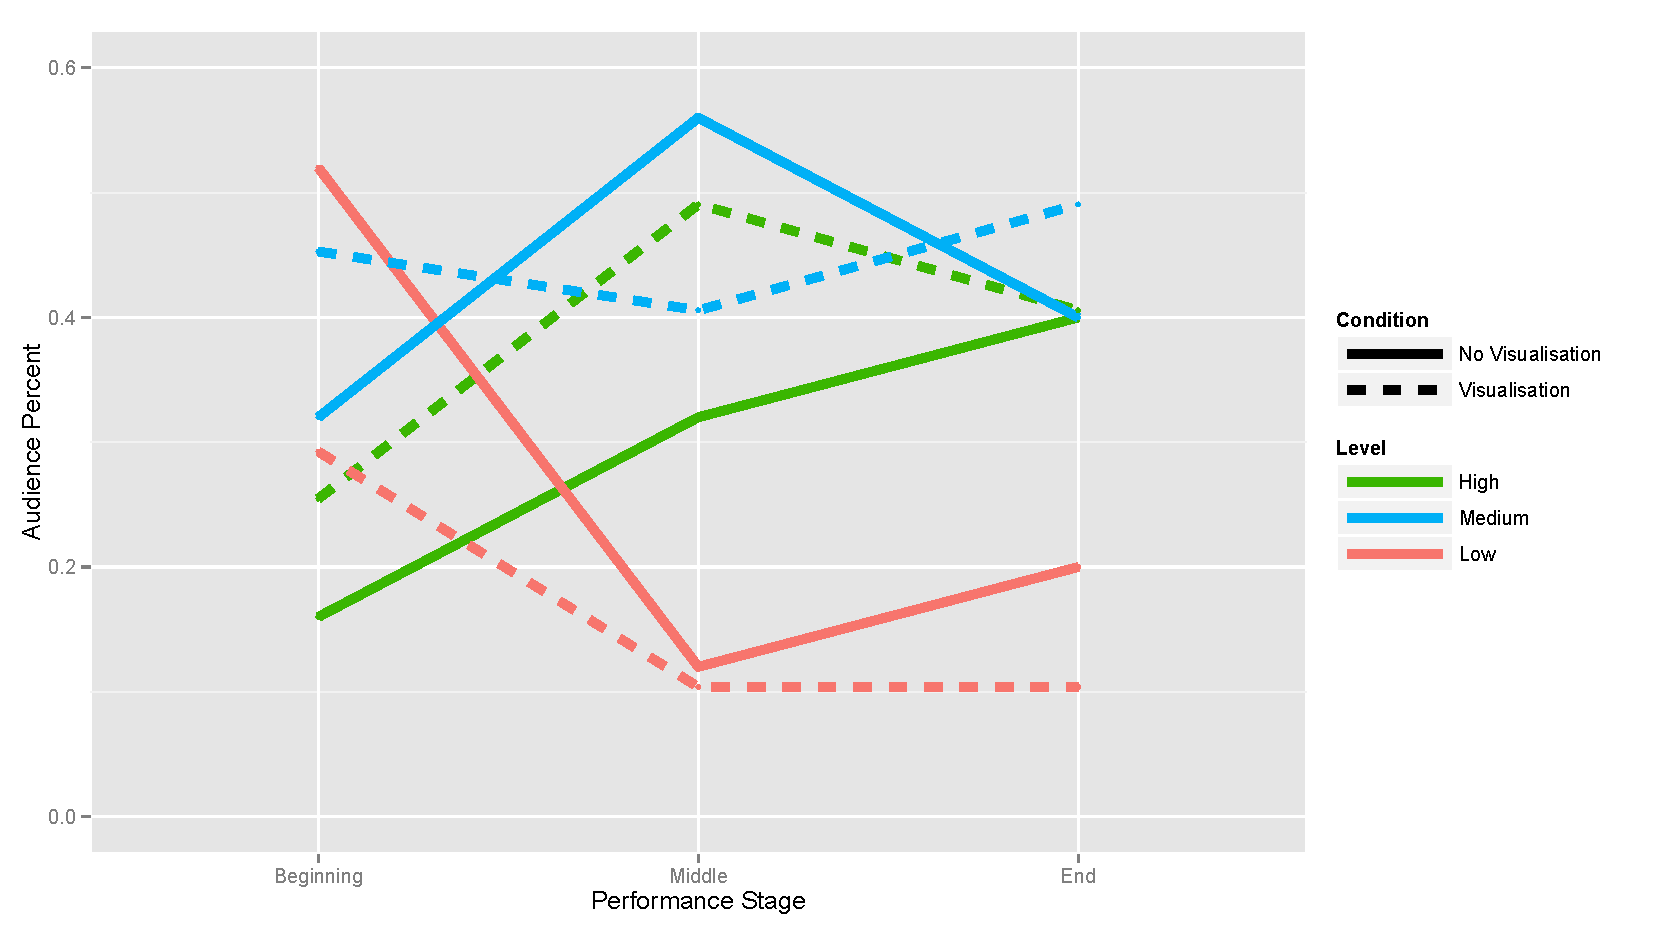
\includegraphics[width=\columnwidth]{../images/graphs/enjoyment-final.pdf}
  \caption{Aggregate comparison of enjoyment within live coding with and without visualisations including results from the intial user study and the follow-up user study.}
  \label{fig:enjoyment-final}
\end{figure}

\begin{figure}
  \centering
  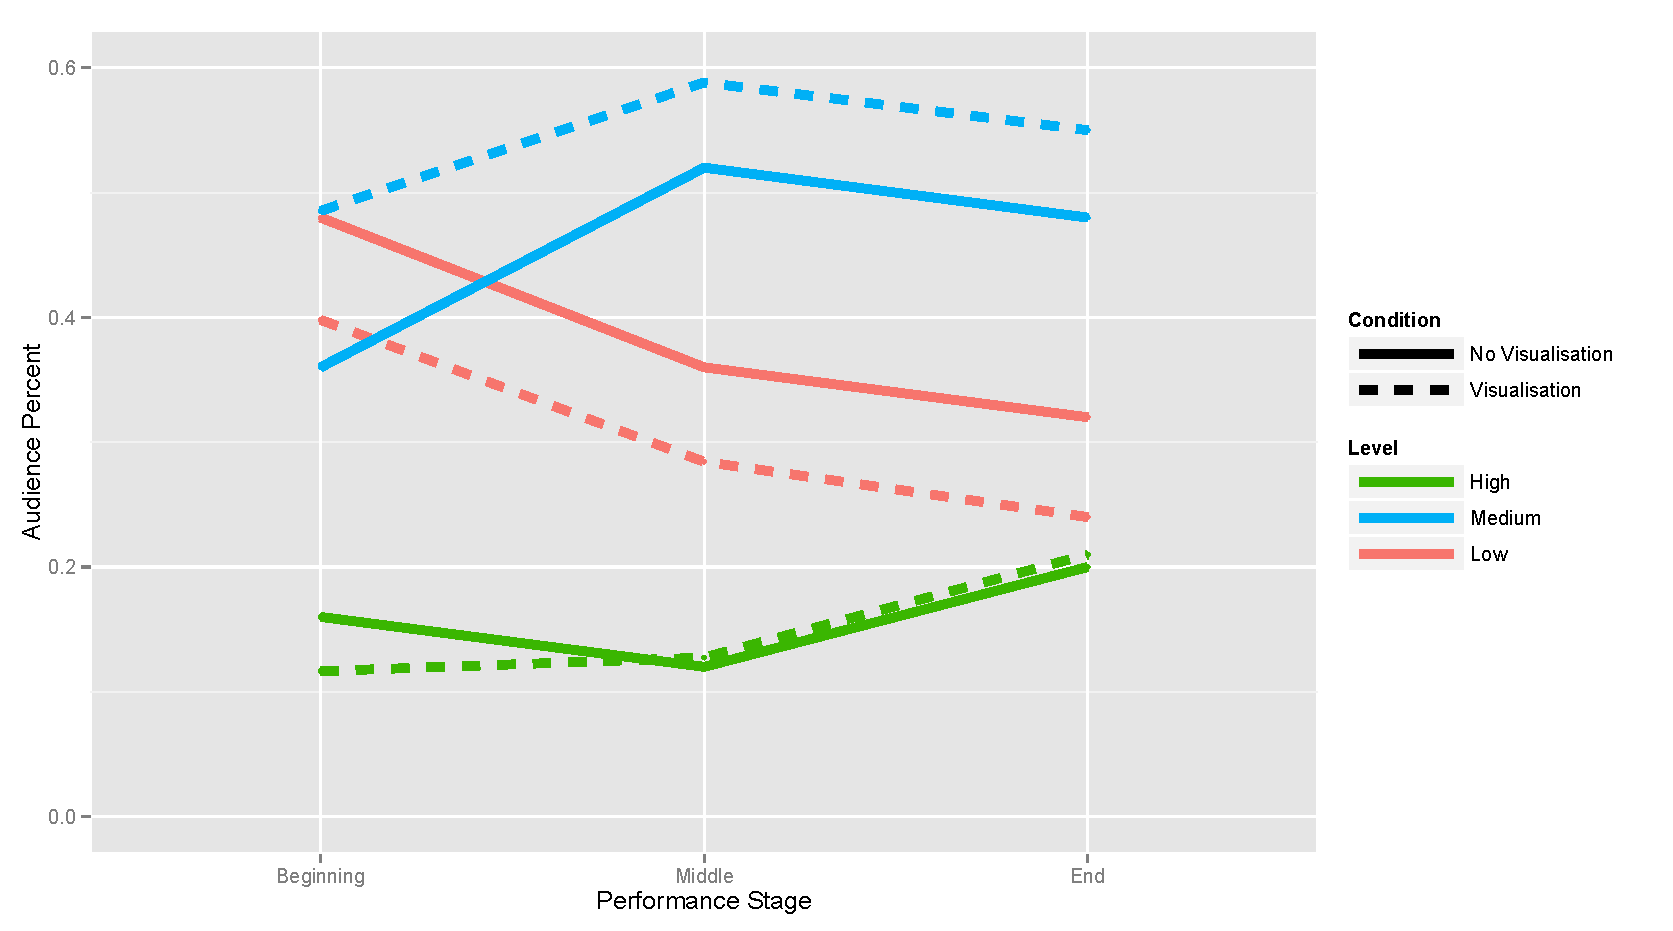
\includegraphics[width=\columnwidth]{../images/graphs/understanding-final.pdf}
  \caption{Aggregate comparison of understanding within live coding with and without visualisations including results from the intial user study and the follow-up user study.}
  \label{fig:understanding-final}
\end{figure}
\clearpage}

From presentation (for Figure~\ref{fig:enjoyment-final}):

[results of this study and the results of previous user study gave rise to the following….]
this graph shows the percent of the audience reporting their levels of enjoyment over the three stages of the performance for the two conditions of “no visualisation” and “with visualisation” 
the no visualisation condition is marked as a solid line
the visualisation condition is marked as a dotted line
the percent of the audience reporting high is marked in green, reporting medium is marked in blue and reporting low is marked in red
a smaller percentage of the low group and a larger percentage of the high group would be desirable

- for example, during the beginning of the performance, for the visualisation condition, 30% of the audience stated that they had low enjoyment while for the no visualisation, 50% of the audience stated that they had low enjoyment

this graph shows an overall increase in enjoyment consistently throughout the performance
increase in a high level of enjoyment with the visualisation, particularly during the middle of the performance
in summary, these results indicate that there is a clear shift upwards in enjoyment throughout the performance, with the visualisations always performing equal or better than the no visualisation condition

From presentation (for Figure~\ref{fig:understanding-final}):

this graph is for understanding and is a similar format to the previous
coloured lines show percent of audience with that level of understanding

shows an increase in the percent reporting medium understanding with the visualisation compared to without… 
visualisations appears to help audiences reporting low understanding
however, little impact on the percent reporting high levels of understanding
-  in summary, it shows a consistent increase throughout the performance for all except those with high understanding



\subsection{Performance Start}

% Content Analysis Questions:
% Which data are analysed?
% How are they defined?
% What is the population from which they are drawn?
% What is the context relative to which the data are analysed?
% What are the boundaries of the analysis?
% What is the target of the inferences?

\subsection{Performance End}


\subsection{Comparison to Previous Study}



\subsection{Validity}

A number of factors were identified that could influence the validity of the user study results.

Due to a technical oversight during the first performance, the visualisation underlay was difficult to distinguish. 
% This was this was intentionally left the same for the second performance group.

A large proportion of the audience stated that they had coding experience. An audience experienced in coding may be less interested in viewing visualisations and have a preference for viewing code directly.

-no significance in the results

Again, musical style... instruments... differences between two performances etc

\more

\subsection{Limitations}

The visualisations again suffered from being obscured by the source code displayed on the projection screen. However, compared to initial user study, the visualisations were logically placed in relation to the source code, from top to bottom, in the order the functions appeared in the code.

\section{Summary}

This study 
\more








